
%This is a template for producing reports for "Dagstuhl Reports".
%See dagrep-v2021.pdf for further information.

\documentclass[a4paper,UKenglish]{dagrep-v2021}
  %for A4 paper format use option "a4paper", for US-letter use option "letterpaper"
  %for british hyphenation rules use option "UKenglish", for american hyphenation rules use option "USenglish"
  %for section-numbered lemmas etc., use "numberwithinsect"
  %for producing a PDF according the PDF/A standard, add "pdfa"

\usepackage{microtype}%if unwanted, comment out or use option "draft"
\pdfoutput=1
\usepackage[utf8]{inputenc}
\usepackage{amsmath}
\usepackage{amssymb}
\usepackage{mathpartir}
\usepackage{hyperref}
\usepackage{listings}
\usepackage{graphicx}
\usepackage{comment}
\usepackage{todonotes}
\newcommand\pt{\todo[author=PT,inline]}
\lstdefinelanguage{michelson}{
  basicstyle=\fontsize{8}{9.6}\selectfont,
  morekeywords={parameter,storage,or,unit,mutez,pair,bool,address}, sensitive=false,
  morecomment=[l]{\#},
  morecomment=[\STACK]{/*}{*/},
  morestring=[b]",
}
\lstset{
  language=Caml,
  captionpos=b,
  aboveskip=-\smallskipamount,
  belowskip=-\smallskipamount,
  belowcaptionskip=0pt,
  basicstyle=\fontsize{8}{9.6}\selectfont,
  morekeywords={val}
}

%% structure
\newcommand{\Angle}[1]{\langle#1\rangle}

%% values
\newcommand{\NEG}{\neg}
\newcommand{\CNF}{\wedge}
\newcommand{\DNF}{\vee}
\newcommand{\TRUE}{\text{True}}
\newcommand{\FALSE}{\text{False}}
\newcommand{\EMPTYSTRING}{\text{$""$}}
\newcommand{\STACKCONCAT}{\text{$::$}}
\newcommand{\ZERO}{\text{0}}
\newcommand{\ONE}{\text{1}}
\newcommand{\VAMOUNT}{\text{amount}}
\newcommand{\VCONTRACT}{\text{contract}}

%% contract constants
\newcommand{\CAMOUNT}{\text{amount}}
\newcommand{\CBALANCE}{\text{balance}}
\newcommand{\CSENDER}{\text{sender}}
\newcommand{\CSOURCE}{\text{source}}
\newcommand{\CNOW}{\text{now}}
\newcommand{\CLEVEL}{\text{level}}
\newcommand{\CCHAINID}{\text{chain-id}}
\newcommand{\CSELF}{\text{self}}
\newcommand{\CSELFADDRESS}{\text{self-address}}
\newcommand{\CTOTALVOTINGPOWER}{\text{total-voting-power}}
\newcommand{\CVOTINGPOWER}{\text{voting-power}}

%% contract instructions
\newcommand{\AMOUNT}{\text{AMOUNT}}
\newcommand{\BALANCE}{\text{BALANCE}}
\newcommand{\SENDER}{\text{SENDER}}
\newcommand{\SOURCE}{\text{SOURCE}}
\newcommand{\NOW}{\text{NOW}}
\newcommand{\LEVEL}{\text{LEVEL}}
\newcommand{\CHAINID}{\text{CHAIN-ID}}
\newcommand{\SELF}{\text{SELF}}
\newcommand{\SELFADDRESS}{\text{SELF-ADDRESS}}
\newcommand{\TOTALVOTINGPOWER}{\text{TOTAL-VOTING-POWER}}
\newcommand{\VOTINGPOWER}{\text{VOTING-POWER}}
\newcommand{\MinusBalanceAmount}{\text{BALANCE-AMOUNT}}
%% auction contract
\newcommand{\AuctionOwner}{\text{auction-owner}}
\newcommand{\AuctionBidder}{\text{auction-bidder}}
\newcommand{\AuctionClose}{\text{auction-close}}
\newcommand{\AuctionOpen}{\text{auction-open}}
\newcommand{\AuctionBid}{\text{auction-bid}}

%% system definition
\newcommand{\VAL}{\textbf{v}}
\newcommand{\VAR}{\textbf{x}}
\newcommand{\VARIABLE}{\text{$Var$}}
\newcommand{\CONSTANT}{\text{$Const$}}
\newcommand{\TERM}{\text{$T$}}
\newcommand{\VariableX}{\text{$x$}}
\newcommand{\VariableV}{\text{$v$}}
\newcommand{\VariableK}{\text{$k$}}
\newcommand{\VariableA}{\text{$a$}}
\newcommand{\VariableB}{\text{$b$}}
\newcommand{\ELT}{\text{$Elt$}}
\newcommand{\A}{\text{$A$}}
\newcommand{\B}{\text{$B$}}
\newcommand{\N}{\text{$n$}}
\newcommand{\K}{\text{$k$}}
\newcommand{\V}{\text{$v$}}
\newcommand{\M}{\text{$m$}}
\newcommand{\VariableOne}{\text{$x_1$}}
\newcommand{\VariableTwo}{\text{$x_2$}}
\newcommand{\VariableN}{\text{$x_n$}}
\newcommand{\Constant}{\text{$c$}}
\newcommand{\ConstantOne}{\text{$c_1$}}
\newcommand{\ConstantTwo}{\text{$c_2$}}
\newcommand{\ConstantN}{\text{$c_n$}}
\newcommand{\LIST}{\text{$l$}}
\newcommand{\EMPTYLIST}{\text{$\{\}$}}
\newcommand{\TLIST}{\text{$l'$}}
\newcommand{\HEAD}{\text{$hd$}}
\newcommand{\TAIL}{\text{$tl$}}
\newcommand{\STAIL}{\text{$< tl >$}}
\newcommand{\Term}{\text{$t$}}
\newcommand{\TermOne}{\text{$t_1$}}
\newcommand{\TermTwo}{\text{$t_2$}}
\newcommand{\TermN}{\text{$t_n$}}
\newcommand{\TermB}{\text{$t_b$}}
\newcommand{\STACK}{\text{$S$}}
\newcommand{\EMPTYSTACK}{\text{[ ]}}
\newcommand{\STACKONE}{\text{$S$}}
\newcommand{\STACKTWO}{\text{$S$}}
\newcommand{\STACKN}{\text{$S$}}
\newcommand{\Stack}{\text{$s$}}
\newcommand{\StackOne}{\text{$s_1$}}
\newcommand{\StackTwo}{\text{$s_2$}}
\newcommand{\StackN}{\text{$s_n$}}
\newcommand{\TSTACK}{\text{$S'$}}
\newcommand{\TStack}{\text{$s'$}}
\newcommand{\STATE}{\text{$ST$}}
\newcommand{\STATEONE}{\text{$ST_1$}}
\newcommand{\STATETWO}{\text{$ST_2$}}
\newcommand{\STATEN}{\text{$ST_n$}}
\newcommand{\SYSTEM}{\text{$SE$}}
\newcommand{\INSTRUCTION}{\text{$I$}}
\newcommand{\TINSTRUCTION}{\text{$I'$}}
\newcommand{\INSTRUCTIONONE}{\text{$I1$}}
\newcommand{\INSTRUCTIONTWO}{\text{$I2$}}
\newcommand{\Instruction}{\text{$i$}}
\newcommand{\TInstruction}{\text{$i'$}}
\newcommand{\InstructionOne}{\text{$i_1$}}
\newcommand{\InstructionTwo}{\text{$i_2$}}
\newcommand{\InstructionN}{\text{$i_n$}}
\newcommand{\Invariant}{\text{$Iv$}}
\newcommand{\PREDICATE}{\text{$P$}}
\newcommand{\PREDICATEA}{\text{$P_A$}}
\newcommand{\PREDICATEB}{\text{$P_B$}}
\newcommand{\Predicate}{\text{$p$}}
\newcommand{\Failwith}{\text{$Failwith$}}
\newcommand{\PredicateOne}{\text{$p_1$}}
\newcommand{\PredicateTwo}{\text{$p_2$}}
\newcommand{\PredicateN}{\text{$p_n$}}
\newcommand{\SETA}{\text{$\mathcal{A}$}}
\newcommand{\SETAAUCTION}{\text{$\mathcal{A}_{auction}$}}
\newcommand{\SETPOST}{\text{$\mathcal{A'}$}}
\newcommand{\SETPOSTAUCTION}{\text{$\mathcal{A'}_{auction}$}}
\newcommand{\EMPTY}{\text{$\O$}}
\newcommand{\PCreate}{\text{$P_{Create}$}}
\newcommand{\PBidding}{\text{$P_{Bidding}$}}
\newcommand{\PClose}{\text{$P_{Close}$}}
\newcommand{\SE}{\text{SE}}
\newcommand{\SINIT}{\text{$s_{init}$}}
\newcommand{\SFINAL}{\text{$s_{final}$}}
\newcommand{\FMAP}{\textbf{map}}
\newcommand{\MAPA}{\textbf{$map_A$}}
\newcommand{\MAPB}{\textbf{$map_B$}}
\newcommand{\MapBidding}{\textbf{$map_{bidding}$}}
\newcommand{\MapCreate}{\textbf{$map_{create}$}}
\newcommand{\MapClose}{\textbf{$map_{close}$}}
\newcommand{\MAPER}{\text{$\overline{\textbf{map}}$}}


%% operation
\newcommand{\CONS}{\text{cons}}
\newcommand{\NIL}{\text{nil}}
\newcommand{\PLUS}{\textbf{+}}
\newcommand{\MINUS}{\textbf{-}}
\newcommand{\EQUAL}{\textbf{=}}
\newcommand{\LESS}{\textbf{$<$}}
\newcommand{\LESSEQUAL}{\textbf{$<=$}}
\newcommand{\MORE}{\textbf{$>$}}
\newcommand{\MOREEQUAL}{\textbf{$>=$}}

%% instructions
\newcommand{\UNIT}{\text{Unit}}
\newcommand{\PAIR}{\text{Pair}}
\newcommand{\LEFT}{\text{Left}}
\newcommand{\RIGHT}{\text{Right}}
\newcommand{\SOME}{\text{Some}}
\newcommand{\NONE}{\text{None}}
\newcommand{\ADD}{\text{ADD}}
\newcommand{\DROP}{\text{DROP}}
\newcommand{\LOOP}{\text{LOOP}}
\newcommand{\FAILWITH}{\text{FAILWITH}}
\newcommand{\TRANSFER}[2]{\text{Transfer($#1$, $#2$)}}
\newcommand{\CONTRACT}{\text{CONTRACT}}
\newcommand{\CAR}{\text{CAR}}
\newcommand{\EXEC}{\text{EXEC}}
\newcommand{\APPLY}{\text{APPLY}}
\newcommand{\IF}{\text{IF}}
\newcommand{\IFLEFT}{\text{IF-LEFT}}
\newcommand{\IFRIGHT}{\text{IF-RIGHT}}
\newcommand{\IFCONS}{\text{IF-CONS}}
\newcommand{\ITER}{\text{ITER}}
\newcommand{\TITER}{\text{ITER'}}
\newcommand{\DIG}{\text{DIG}}
\newcommand{\DIP}{\text{DIP}}
\newcommand{\DIPN}{\text{DIP n}}
\newcommand{\TDIP}{\text{DIP'}}
\newcommand{\ABS}{\text{ABS}}
\newcommand{\COMPARE}{\text{COMPARE}}
\newcommand{\TCOMPARE}{\text{COMPARE'}}
\newcommand{\HASHKEY}{\text{HASH-KEY}}
\newcommand{\CONCAT}{\text{CONCAT}}
\newcommand{\TCONCAT}{\text{CONCAT'}}
\newcommand{\MEN}{\text{MEN}}
\newcommand{\TMEN}{\text{MEN'}}
\newcommand{\TMAP}{\text{MAP'}}
\newcommand{\PUSH}{\text{PUSH}}
\newcommand{\XOR}{\text{XOR}}
\newcommand{\MAP}{\textbf{MAP}}
\newcommand{\LAMBDA}{\text{LAMBDA}}


%symbols
\newcommand{\Overline}[1]{\text{$\overline{#1}$}}
\newcommand{\Mapsto}{\text{$\mapsto$}}
\newcommand{\Mid}{\text{$\mid$}}
\newcommand{\Mathcal}[1]{\text{$\mathcal{#1}$}}
\newcommand{\Models}{\text{$\models$}}
\newcommand{\SRightarrow}{\text{$\rightarrow$}}
\newcommand{\NSRightarrow}{\text{$\nrightarrow$}}
\newcommand{\Wedge}{\text{$\wedge$}}
\newcommand{\At}{\text{$@$}}
\newcommand{\Subseteq}{\text{$\subseteq$}}
\newcommand{\Vee}{\text{$\vee$}}
%\newcommand{\Cup}{\text{$\cup$}}
\newcommand{\STRINGCONCAT}{\text{$\hat{}$}}
\newcommand{\DOT}{\text{$...$}}


%% functions
\newcommand{\FABS}[1]{\text{abs($#1$)}}
\newcommand{\FXOR}{\text{xor}}
\newcommand{\FHASHKEY}[1]{\text{hash-key($#1$)}}
\newcommand{\FCONCAT}[1]{\text{concat($#1$)}}
\newcommand{\FGetTy}[1]{\text{get-ty($#1$)}}
\newcommand{\FLEN}[1]{\text{len($#1$)}}
\newcommand{\FAND}{\text{and}}
\newcommand{\FOR}{\text{or}}
\newcommand{\FNOT}{\text{not}}
\newcommand{\GETCONTRACTTYPE}{\text{get-contract-type}}
\newcommand{\UNOP}{\text{unop}}
\newcommand{\BINOP}{\text{binop}}



%% transition relations
\newcommand{\StateTrans}{\text{$\longrightarrow_S$}}
\newcommand{\ExprTrans}{\text{$\longrightarrow_E$}}
\newcommand{\SystemTrans}{\text{$\longrightarrow$}}


%% types
\newcommand\TEnv{\Gamma}
\newcommand\JTypeCode[2]{\vdash_C#1 : #2}
\newcommand\JTypeValue[2]{\vdash_V#1 : #2}
\newcommand\JTypeExpr[3]{#1 \vdash #2 : #3}
\newcommand{\TY}{\text{ty}}
\newcommand{\TYF}{\text{ty$_{1}$}}
\newcommand{\TYS}{\text{ty$_{2}$}}
\newcommand{\TYT}{\text{ty$_{3}$}}
\newcommand{\TYA}{\text{A}}
\newcommand{\TYB}{\text{B}}
\newcommand{\TYC}{\text{C}}
%% standard types
\newcommand{\TBOOL}{\text{bool}}
\newcommand{\TOR}{\text{or}}
\newcommand{\TYLIST}{\text{list}}
\newcommand{\TUNIT}{\text{unit}}
\newcommand{\TPAIR}{\text{pair}}
\newcommand{\TOPTION}{\text{option}}
\newcommand{\TMUTEZ}{\text{mutez}}
\newcommand{\TSTR}{\text{string}}
\newcommand{\TINT}{\text{int}}
\newcommand{\TNAT}{\text{nat}}
\newcommand{\TKEY}{\text{key}}
\newcommand{\TKEYHASH}{\text{key-hash}}
\newcommand{\TSIG}{\text{signature}}
\newcommand{\TADDR}{\text{address}}
\newcommand{\TTIME}{\text{timestamp}}
\newcommand{\TCONTRACT}{\text{contract}}
\newcommand{\TCHAINID}{\text{chain-id}}
\newcommand{\TLAMBDA}{\text{lambda}}







%% typing related
\newcommand{\EmptyEnv}{\cdot}

%% evaluation contexts
\newcommand\EC[1]{\epsilon[#1]}

%% metavariables


%%% Local Variables:
%%% mode: latex
%%% TeX-master: "paper"
%%% End:



\bibliographystyle{plain}%the recommnded bibstyle

\subject{Report from Dagstuhl Seminar 11013}
\title{Formal Verification Tool Based on Symbolic Execution for Smart Contract}
\titlerunning{11013 -- Seminar Sample}%optional

\author[1]{Thi Thu Ha Doan}
\author[2]{Peter Thiemann}
\affil[1]{University of Freiburg, Germany
  \texttt{doanha@informatik.uni-freiburg.de}}
\affil[2]{University of Freiburg, Germany
  \texttt{thiemann@informatik.uni-freiburg.de}}
\authorrunning{T.T.H Doan and P.Thiemann}%optional

\keywords{Smart Contract, Blockchain, Formal Verification, Symbolic Execution}%mandatory

%Organizer macros:%%%%%%%%%%%%%%%%%%%%%%%%%%%%%%%%%%%%%%%%%%%%%%%%%%%%%
\seminarnumber{11013}
\semdata{03.--07.~January, 2011 -- \url{https://www.dagstuhl.de/11013}}

\ccsdesc[100]{General and reference~General literature}
\ccsdesc[500]{Hardware~3D integrated circuits}
\ccsdesc[500]{Software and its engineering~Software design engineering}
\ccsdesc[300]{Networks~Network performance analysis}

\additionaleditors{Tom Collector}%optional
%%%%%%%%%%%%%%%%%%%%%%%%%%%%%%%%%%%%%%%%%%%%%%%%%%%%%%%%%%%%%%%%%%%%%%%

%Dagstuhl editorial office macros:%%%%%%%%%%%%%%%%%%%%%%%%%%%%%%%%%%%%%
\volumeinfo%(easychair interface)
  {John Q. Open and Joan R. Access}%editors
  {2}%number of editors
  {Seminar Sample}%event
  {1}%volume
  {1}%issue
  {1}%starting page number
\DOI{10.4230/DagRep.1.1.1}%(DagRep.<issue no>.<volume no>.<firstpage>)
%%%%%%%%%%%%%%%%%%%%%%%%%%%%%%%%%%%%%%%%%%%%%%%%%%%%%%%%%%%%%%%%%%%%%%%

\begin{document}

\maketitle

\begin{abstract}
In the context of blockchain technology, the immutability of smart contracts once implemented underscores the critical need to ensure their accuracy. Even in cases where smart contract implementations are not overly extensive and have undergone testing before deployment, the blockchain community has identified significant vulnerabilities in their design. In addition, the relatively new nature of smart contract languages has led to unforeseen errors due to a lack of familiarity with their intricacies. To overcome these challenges, formal verification emerges as a key solution to guarantee the correctness of smart contracts. In response to this need, we have developed a formal verification tool for smart contracts, particularly those written in Michelson. This tool uses symbolic execution to simulate the implementation of the smart contract language, helping to detect subtle errors that are difficult for smart contract developers to detect. In addition, our tool includes a domain-specific language that allows users to precisely specify contract properties. By interacting with an SMT solver, it can handle a wide range of properties. In particular, it streamlines the process of reviewing requirements, uncovering hidden errors, and validating user-defined properties. In summary, our research highlights the need for robust verification of smart contracts. We present a purpose-built tool that utilizes symbolic execution and a domain-specific language to improve the correctness of smart contracts and provide a comprehensive solution to mitigate potential pitfalls in blockchain-based applications.
\end{abstract}

\summaryauthor[T.T.Ha Doan and P. Thiemann]{%
T.T.Ha Doan (University of Freiburg, Germany, doanha@informatik.uni-freiburg.de)\\
P. Thiemann (University of Freiburg, Germany, \\thiemann@informatik.uni-freiburg.de)
}

\license




\tableofcontents

%\newpage

\section{Introduction}
\label{sec:introduction}

\section{Symblic Execution Model}
\label{sec:symblic-execution-model}

Let $\STACK = (\TermOne, \TYF) \STACKCONCAT (\TermTwo, \TYS) \STACKCONCAT \DOT
\STACKCONCAT \EMPTYSTACK$ be a stack, where elements are types paired with terms.
\\
Let $\INSTRUCTION = \InstructionOne; \InstructionTwo; \DOT; \InstructionN$ be a sequence of instructions. 
\\
Let \PREDICATE\ be a predicate. 

\begin{definition}
A system state of the symbolic execution is a tuple \\ $\STATE = [\INSTRUCTION, \STACK, \PREDICATE]$. Let $\SYSTEM = \{\STATEONE, \STATETWO, \DOT, \STATEN \}$ range over sets of system states.
\end{definition}

Let $S_{init}$   = (\KPAIR\ \VPAR\ \VSTORAGE, \TPAIR\ \TYF\ \TYS) \STACKCONCAT\EMPTYSTACK\ be the initial  stack, where \VPAR\ and \VSTORAGE\ are the terms that represent the parameter and the storage and \TYF\ and \TYS\ are their corresponding types, and  $S_{final}$   = (\PAIR\ \VOPERATIONLIST\ \VSTORAGE, \TPAIR\ (\TOPERATIONLIST) \TYS) \STACKCONCAT\EMPTYSTACK\ be  the final stack, where \VOPERATIONLIST\ repesents a operation list



\begin{figure} []
\begin{align*}
T, U &::= \\
   &\Mid\ \langle \text{comparable type}\rangle \\
   &\Mid\ \text{option}\ \langle\text{type}\rangle \\
   &\Mid\ \text{list}\ \langle\text{type}\rangle \\
   &\Mid\ \text{set}\ \langle\text{comparable type}\rangle \\
   &\Mid\ \text{operation} \\
   &\Mid\ \text{contract}\ \langle\text{type}\rangle \\
   &\Mid\ \text{ticket}\ \langle\text{comparable type}\rangle \\
   &\Mid\ \text{pair}\ \langle\text{type}\rangle \langle\text{type}\rangle \\
   &\Mid\ \text{or}\ \langle\text{type}\rangle \langle\text{type}\rangle \\
   &\Mid\ \text{lambda}\ \langle\text{type}\rangle \langle\text{type}\rangle \\
   &\Mid\ \text{map}\ \langle\text{comparable type}\rangle \langle\text{type}\rangle \\
   &\Mid\ \text{big-map}\ \langle\text{comparable type}\rangle \langle\text{type}\rangle \\
   &\Mid\ \text{bls12-381-g1} \\
   &\Mid\ \text{bls12-381-g2} \\
   &\Mid\ \text{bls12-381-fr} \\
   &\Mid\ \text{sapling-transaction}\ \langle\text{natural number constant}\rangle \\
   &\Mid\ \text{sapling-state}\ \langle\text{natural number constant}\rangle \\
   &\Mid\ \text{chest} \\
   &\Mid\ \text{chest-key} \\
\langle\text{comparable type}\rangle ::= \\
   &\Mid\ \text{unit} \\
   &\Mid\ \text{never} \\
   &\Mid\ \text{bool} \\
   &\Mid\ \text{int}\\
   &\Mid\ \text{nat}\\
   &\Mid\ \text{string}\\
   &\Mid\ \text{chain-id}\\
   &\Mid\ \text{bytes}\\
   &\Mid\ \text{mutez}\\
   &\Mid\ \text{key-hash}\\
   &\Mid\ \text{key}\\
   &\Mid\ \text{signature}\\
   &\Mid\ \text{timestamp}\\
   &\Mid\ \text{address}\\
   &\Mid\ \text{tx-rollup-l2-address}\\
   &\Mid\ \text{option}\ \langle\text{comparable type}\rangle\\
   &\Mid\ \text{or}\ \langle\text{comparable type}\rangle \langle\text{comparable type}\rangle\\
   &\Mid\ \text{pair}\ \langle\text{comparable type}\rangle \langle\text{comparable type}\rangle \DOT \\
\end{align*}
\caption{Types}
\label{fig:type}
\end{figure}

\begin{figure}[h]
\begin{align*}
\text{t} &::= \\
   &\Mid\ \langle \text{variable} \rangle \\
   &\Mid\ \langle \text{account constant} \rangle \\
   &\Mid\ \langle \text{int constant} \rangle \\
   &\Mid\ \langle \text{string constant} \rangle \\
   &\Mid\ \langle \text{byte sequence constant} \rangle \\
   &\Mid\ \UNIT \\
   &\Mid\ \TRUE \\
   &\Mid\ \FALSE \\
   &\Mid\ \PAIR\ \text{t1 t2}\\
   &\Mid\ \LEFT\ \text{t}\\
   &\Mid\ \RIGHT\ \text{t}\\ 
   &\Mid\ \SOME\ \text{t}\\
   &\Mid\ \NONE \\
   &\Mid\ \text{\{t ; ... \}}\\
   &\Mid\ \text{\{ Elt t1 t2 ; ... \}}\\
   &\Mid\ \{ \langle\text{instruction}\rangle; ... \}   \\
\langle \text{variable} \rangle &::= \\ 
   &\Mid\ \VAR\\
\langle \text{account constant} \rangle &::= \\ 
   &\Mid\ \text{balance} \\
   &\Mid\ \text{amount} \\
   &\Mid\ \text{sender} \\
   &\Mid\ \text{source} \\
   &\Mid\ \text{now} \\
   &\Mid\ \text{level} \\
   &\Mid\ \text{chain-id} \\
   &\Mid\ \text{self}  \\
   &\Mid\ \text{self-address}  \\
   &\Mid\ \text{total-voting-power}  \\
   &\Mid\ \text{voting-power}  \\
\langle \text{natural number constant} \rangle &::= \\ 
   &\Mid\ \text {[0-9]+} \\
\langle \text{int constant} \rangle &::= \\
  &\Mid\ \langle \text{natural number constant} \rangle \\
  &\Mid\ \text{-} \langle \text{natural number constant} \rangle \\
\langle\text{string constant}\rangle &::= \\
  &\Mid\ \text{"} \langle \text{string content}\rangle\text{*"} \\
\langle\text{instruction}\rangle &::= \\
  &\Mid\ \DROP \\
  &\Mid\ \DROP \langle\text{natural number constant}\rangle \\
  &\text{...}
\end{align*}
\caption{Terms}
\label{fig:term}
\end{figure}


\begin{figure}[h]
\begin{align*}
\text{p} &::= \\
   &\Mid\ \langle \text{atomic formula} \rangle \\
   &\Mid\ \NEG\ \text{p} \
   \Mid\ \text{p}\ \CNF\ \text{q} \
   \Mid\ \text{p}\ \DNF\ \text{q} \\
\langle \text{atomic formula} \rangle &::= \\ 
    &\Mid\ \langle \text{butop} \rangle \langle \text{bterm} \rangle\\ 
   &\Mid\  \langle \text{bterm} \rangle  \langle \text{biop} \rangle \langle \text{bterm} \rangle\\ 
\langle \text{butop} \rangle &::= \\
   &\Mid\ \text{not} \\
\langle \text{biop} \rangle &::= \\
   &\Mid\ \text{$=$} \
   \Mid\ \text{$>$} \
   \Mid\ \text{$<$} \
   \Mid\ \text{$>=$} \
   \Mid\ \text{$=<$} \
   \Mid\ \text{$!=$} \\
   &\Mid\ \text{and}\ \Mid\ \text{or}\ \Mid\ \text{xor}\\
\langle \text{bterm} \rangle &::= \\ 
   &\Mid\ \text{t} \\
   &\Mid\ \langle \text{unop} \rangle \text{t} \\ 
   &\Mid\ \text{t}\ \langle \text{binop} \rangle \text{t}\\  
\langle \text{unop} \rangle &::= \\ 
   &\Mid\ \text{abs} \\
   &\Mid\ \text{size} \\
   &\Mid\ \text{int} \\
   &\Mid\ \text{contract}  \langle \text{type} \rangle \\
   &\Mid\ \text{isleft} \\
   &\Mid\ \text{isnone} \\
   &\Mid\ \text{neg} \\
   &\Mid\ \text{blake2b} \\
   &\Mid\ \text{hash-key} \\
   &\Mid\ \text{keccak} \\
   &\Mid\ \text{pairing-check} \\
   &\Mid\ \text{sha256} \\
   &\Mid\ \text{sha3} \\
   &\Mid\ \text{sha512} \\
   &\Mid\ \text{implicit-account} \\
   &\Mid\ \text{check-sig} \\
\langle \text{bitop} \rangle &::= \\ 
   &\Mid\ \text{+}\ \Mid\ \text{-}\ \Mid\ \text{*}\ \Mid\ \text{/}
\end{align*}
\caption{Predicates}
\label{fig:predicate}
\end{figure}


%\paragraph{Sequence actions.}
%\begin{figure}[h]
%\center
%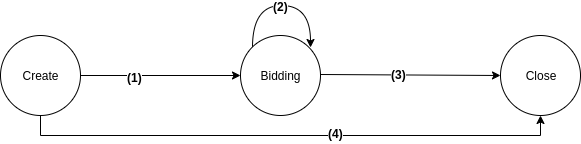
\includegraphics[width= 10 cm]{life-cycle-1}
%\caption{Life-cycle for the auction contract.}
%\label{fca1}
%\end{figure} 

\pagebreak
\subsection{Rules}
The rule semantic is defined by several kinds of transitions:
\begin{enumerate}
\item \ExprTrans\ single-step evaluation of an expression in a system state,
\item \StateTrans\ internal transitions of a system state, which is non-deterministic  as shown for instructions \LOOP\ and \LOOP-LEFT,
\item \SystemTrans\ symbolic system transitions.
\end{enumerate}

\subsubsection{System rules}
\begin{mathpar}
\inferrule[INVALID-PRE]
  { \NEG\ \PREDICATE
  }{
  \{[\INSTRUCTION, \STACK, \PREDICATE]\} \cup \SYSTEM \SystemTrans \SYSTEM}
\end{mathpar}

\subsubsection{Instruction rules}
\paragraph{Control structures}
%EXE
\begin{mathpar}
  \inferrule[EXEC]
  {
    [\INSTRUCTIONONE, (\StackOne, \TYF) \STACKCONCAT \EMPTYSTACK, 
    Q]
    \StateTrans^*
    [ \EMPTYSTACK, (\StackOne', \TYS) \STACKCONCAT Q']
  }{
     [(\EXEC; \INSTRUCTION),   (\{\INSTRUCTIONONE\}, \TYF\ \rightarrow\ \TYS) \STACKCONCAT
    (\StackOne, \TYF) \STACKCONCAT \STACK, \PREDICATE \wedge Q] 
    \StateTrans \
    [ \INSTRUCTION, (\StackOne', \TYS) \STACKCONCAT \STACK,
    \PREDICATE \wedge Q']}
\end{mathpar}

%APPLY
\begin{mathpar}
  \inferrule[APPLY]
  {
  }{
    [(\APPLY; \INSTRUCTION), (\StackOne, \TYF) \STACKCONCAT(\{\INSTRUCTIONONE\}, \TLAMBDA\ (\TPAIR\ \TYF\  \TYS)\ \TYT) \STACKCONCAT\STACK, \PREDICATE] \StateTrans\\ [\INSTRUCTION, (\{\PUSH\ \TYF\ \StackOne; \IPAIR; \INSTRUCTIONONE\}, \TLAMBDA\ \TYS\ \TYT ) \STACKCONCAT\STACK, \PREDICATE]}
\end{mathpar}

%LAMBLA
\begin{mathpar}
  \inferrule[LAMBDA]
  {  
  }{
    [(\LAMBDA\ \TYF\ \TYS\ \{ \INSTRUCTIONONE \} ; \INSTRUCTION),\STACK, \PREDICATE] \StateTrans\ [\INSTRUCTION, (\{\INSTRUCTIONONE\}, \TLAMBDA\ \TYF\ \rightarrow\ \TYS) \STACKCONCAT\STACK, \PREDICATE]}
\end{mathpar}

%IF
\begin{mathpar}
  \inferrule[IF-true]
  {  
  }{
    [(\IF\ \INSTRUCTIONONE\  \INSTRUCTIONTWO; \INSTRUCTION),
    (\StackOne, \TBOOL) \STACKCONCAT\STACK, \PREDICATE]
    \StateTrans\
    [\INSTRUCTIONONE, \STACK, \PREDICATE\ \Wedge\ \StackOne]
  }

  \inferrule[IF-false]
  {  
  }{
    [(\IF\ \INSTRUCTIONONE\  \INSTRUCTIONTWO; \INSTRUCTION),
    (\StackOne, \TBOOL) \STACKCONCAT\STACK, \PREDICATE]
    \StateTrans\
   [\INSTRUCTIONTWO, \STACK, \PREDICATE\ \Wedge\ \NEG\
   \StackOne]
 }
\end{mathpar}


%IF-LEFT-LEFT
\begin{mathpar}
  \inferrule[IF-LEFT-left]
  {  
  }{
    [(\IFLEFT\ \INSTRUCTIONONE\ \INSTRUCTIONTWO; \INSTRUCTION),
    (\StackOne, \TOR\ \TYF\ \TYS) \STACKCONCAT \STACK, \PREDICATE]
    \StateTrans \
    [\INSTRUCTIONONE, (\VariableX, \TYF) \STACKCONCAT\STACK,
    \PREDICATE \wedge (\StackOne\ \EQUAL\ \LEFT\ \VariableX)]
  }
\end{mathpar}

%IF-LEFT-RIGHT
\begin{mathpar}
  \inferrule[IF-LEFT-right]
  {  
  }{
    [(\IFLEFT\ \INSTRUCTIONONE\  \INSTRUCTIONTWO; \INSTRUCTION),
    (\StackOne, \TOR\ \TYF\ \TYS) \STACKCONCAT \STACK, \PREDICATE]
    \StateTrans \
    [\INSTRUCTIONTWO, (\VariableX, \TYS) \STACKCONCAT\STACK, \PREDICATE \wedge (\StackOne\ \EQUAL\ \RIGHT\ \VariableX))]
  }
\end{mathpar}



%IF_CONS
\begin{mathpar}
  \inferrule[IF-CONS-empty]
  {  
  }{
    [(\IFCONS\ \INSTRUCTIONONE\  \INSTRUCTIONTWO; \INSTRUCTION),  (\StackOne, \TYLIST\ \TY) \STACKCONCAT\STACK, \PREDICATE] \StateTrans\  [\INSTRUCTIONTWO; \INSTRUCTION, \STACK, \PREDICATE\ \Wedge\ (\StackOne\ \EQUAL\ \EMPTYLIST)]}
\end{mathpar}

\begin{mathpar}
  \inferrule[IF-CONS-nonempty]
  {  
  }{
   [(\IFCONS\ \INSTRUCTIONONE\  \INSTRUCTIONTWO; \INSTRUCTION),  (\StackOne, \TYLIST\ \TY) \STACKCONCAT\STACK, \PREDICATE], \SYSTEM\ \StateTrans\  \\ [\INSTRUCTIONONE, (\HEAD, \TY) \STACKCONCAT(\{ \TAIL \}, \TYLIST\ \TY) \STACKCONCAT\STACK, \PREDICATE\ \Wedge\ ( \StackOne\ \EQUAL\ \{\HEAD; \STAIL \})]}
\end{mathpar}



%IF_NON
\begin{mathpar}
  \inferrule[IF-NONE-none]
  {  
  }{
    [(\IFNONE\ \INSTRUCTIONONE\  \INSTRUCTIONTWO; \INSTRUCTION),  (\StackOne, \TOPTION\ \TY) \STACKCONCAT\STACK, \PREDICATE], \SYSTEM\ \StateTrans\   [\INSTRUCTIONONE; \INSTRUCTION, \STACK, \PREDICATE\ \Wedge\ (\StackOne\ \EQUAL\ \NONE)]}
\end{mathpar}

\begin{mathpar}
  \inferrule[IF-NONE-some]
  {  
  }{
    [(\IFNONE\ \INSTRUCTIONONE\  \INSTRUCTIONTWO; \INSTRUCTION),   (\StackOne, \TOPTION\ \TY) \STACKCONCAT\STACK, \PREDICATE], \SYSTEM\ \StateTrans\   [\INSTRUCTIONTWO,  (\VariableX, \TY) \STACKCONCAT\STACK, \PREDICATE\ \Wedge\ ( \StackOne\ \EQUAL\ \SOME\ \VariableX)]}
\end{mathpar}


%LOOP
\begin{mathpar}
  \inferrule[LOOP-true]
  {  
  }{
    [(\LOOP\ \INSTRUCTIONONE; \INSTRUCTION),  (\StackOne, \TBOOL)
    \STACKCONCAT\STACK, \PREDICATE]
    \StateTrans\
    [(\INSTRUCTIONONE; \LOOP\ \INSTRUCTIONONE; \INSTRUCTION),
    \STACK, \PREDICATE \wedge \StackOne]
  }

  \inferrule[LOOP-false]
  {  
  }{
    [(\LOOP\ \INSTRUCTIONONE; \INSTRUCTION),  (\StackOne, \TBOOL) \STACKCONCAT\
    \STACK, \PREDICATE]
    \StateTrans\
   [\INSTRUCTION, \STACK, \PREDICATE \wedge
   (\NEG\StackOne)]
   }
\end{mathpar}

%%ITER
\begin{mathpar}
  \inferrule[ITER-empty]
  {  
  }{
    [(\ITER\ \INSTRUCTIONONE ; \INSTRUCTION), (\StackOne, \TYLIST\ \TY) \STACKCONCAT\STACK, \PREDICATE] \StateTrans\ [\INSTRUCTION, \STACK,  \PREDICATE\ \Wedge\  (\StackOne\ \EQUAL\ \EMPTYLIST)]
  }
\end{mathpar}

\begin{mathpar}
  \inferrule[ITER-nonempty]
  {  [\ITER,  (\HEAD, \TY) \STACKCONCAT\STACK, 
    Q]
    \StateTrans^*
    [ \EMPTYSTACK,  \STACK', Q']
  }{
    [(\ITER\ \INSTRUCTIONONE ; \INSTRUCTION), (\StackOne, \TYLIST\ \TY) \STACKCONCAT\STACK, \PREDICATE \wedge Q] \StateTrans \\ [(\ITER\ \INSTRUCTIONONE ; \INSTRUCTION), \{\STAIL\}\ \STACKCONCAT\STACK',  \PREDICATE \wedge Q' \Wedge  ( \StackOne\ \EQUAL\ \{\HEAD; \STAIL \}) ]
  }
\end{mathpar}


\paragraph{Stack Manipulation}
%DIG
\begin{mathpar}
\inferrule[DIG]
  {
   \FLEN(\A) \EQUAL\ \N
  }
  {[(\DIG\ \N ; \INSTRUCTION), \A\ \At\ (\StackOne, \TY) \STACKCONCAT\B, \PREDICATE] \StateTrans 
[\INSTRUCTION, (\StackOne, \TY) \STACKCONCAT\A\ \At\ \B, \PREDICATE]}
\end{mathpar}

%DIP
\begin{mathpar}
  \inferrule[DIP]
  {
    [\INSTRUCTIONONE,  \STACK, Q]
    \StateTrans^*
    [\EMPTYSTACK,  \STACK_1, Q']
  }
  {[(\DIP\ \INSTRUCTIONONE; \INSTRUCTION), (\StackOne, \TY) \STACKCONCAT
    \STACK, \PREDICATE \wedge Q]
    \StateTrans 
    [\INSTRUCTION, (\StackOne, \TY) \STACKCONCAT\STACK_1,
    \PREDICATE \wedge Q']
  }
\end{mathpar}

%DIP n
\begin{mathpar}
\inferrule[DIP n]
  { 
     \FLEN(\A) \EQUAL\ \N \\ [\INSTRUCTIONONE,  \B, Q]
    \StateTrans^*
    [\EMPTYSTACK,  \B_1, Q']
  }
  {[(\DIP\ \N\ \INSTRUCTIONONE; \INSTRUCTION), \A\ \At\ \B, \PREDICATE \wedge Q] \StateTrans 
[(\INSTRUCTION), \A\ \At\ \B_1, \PREDICATE \wedge Q']}
\end{mathpar}

%PUSH
\begin{mathpar}
  \inferrule[PUSH]
  {  
  }{
    [(\PUSH\ \TY\ \VariableX; \INSTRUCTION),\STACK, \PREDICATE] \StateTrans\ [\INSTRUCTION, (\VariableX, \TY) \STACKCONCAT\STACK, \PREDICATE]}
\end{mathpar}


\paragraph{Arithmetic operations}
%ADD
\begin{mathpar}
\inferrule[ADD]
  {
  }
  {[(\ADD; \INSTRUCTION), (\StackOne, \TNAT) \STACKCONCAT(\StackTwo, \TNAT) \STACKCONCAT\STACK, \PREDICATE] \StateTrans \
[\INSTRUCTION, (\VariableX, \TNAT) \STACKCONCAT\STACK, \PREDICATE \Wedge\ (\VariableX\ \EQUAL\ \StackOne\ \PLUS\ \StackTwo)]}
\end{mathpar}

%ABS
\begin{mathpar}
\inferrule[ABS]
  {
  }
  {
    [(\ABS; \INSTRUCTION), (\StackOne, \TINT) \STACKCONCAT \STACK,
    \PREDICATE]
    \StateTrans \
    [\INSTRUCTION, (\VariableX, \TNAT) \STACKCONCAT \STACK,
    \PREDICATE \wedge (\StackOne \ge 0 \Rightarrow \VariableX =
    \StackOne) \wedge (\StackOne <0 \Rightarrow \VariableX = -\StackOne)]
 }
\end{mathpar}

% COMPARE
\begin{mathpar}
\inferrule[COMPARE-nat]
  {
  }
  {
    [(\COMPARE ; \INSTRUCTION), (\StackOne, \TNAT) \STACKCONCAT (\StackTwo, \TNAT)
    \STACKCONCAT \STACK, \PREDICATE ]
    \SystemTrans \\
    [\INSTRUCTION, (\VariableX, \TINT) \STACKCONCAT \STACK, \PREDICATE
    \wedge\ (\StackOne > \StackTwo \Leftrightarrow \VariableX = 1)
    \wedge\ (\StackOne = \StackTwo \Leftrightarrow \VariableX = 0) 
    \wedge\ (\StackOne < \StackTwo \Leftrightarrow \VariableX = -1)]
    }
\end{mathpar}

\begin{mathpar}
\inferrule[COMPARE-some-some]
  {
  [\COMPARE,  (\VariableX, \TY) \STACKCONCAT (\VariableY, \TY) \STACKCONCAT\EMPTYSTACK, Q]
    \StateTrans^*
    [\EMPTYSTACK,  (\VariableA, \TINT) \STACKCONCAT\EMPTYSTACK, Q']
  }
  {
    [(\COMPARE ; \INSTRUCTION), (\StackOne, \TOPTION\ \TY) \STACKCONCAT (\StackTwo, \TOPTION\ \TY)
    \STACKCONCAT \STACK, \PREDICATE \wedge Q]
    \SystemTrans \\
    [\INSTRUCTION, (\VariableA, \TINT) \STACKCONCAT \STACK,  \PREDICATE
    \wedge (\StackOne\ \EQUAL\ \SOME\ \VariableX)
    \wedge (\StackTwo\ \EQUAL\ \SOME\ \VariableY)
    \wedge Q']
    }
\end{mathpar}

\begin{mathpar}
\inferrule[COMPARE-some-none]
  {
  }
  {
    [(\COMPARE ; \INSTRUCTION), (\StackOne, \TOPTION\ \TY) \STACKCONCAT (\StackTwo, \TOPTION\ \TY)
    \STACKCONCAT \STACK, \PREDICATE]
    \SystemTrans \\
    [\INSTRUCTION, (1, \TINT) \STACKCONCAT \STACK,  \PREDICATE
    \wedge (\StackOne\ \EQUAL\ \SOME\ \VariableX)
    \wedge (\StackTwo\ \EQUAL\ \NONE)
    ]
    }
\end{mathpar}

\paragraph{Boolean operations}
%XOR
\begin{mathpar}
\inferrule[XOR]
  {
  }
  {[(\XOR; \INSTRUCTION), (\StackOne, \TBOOL) \STACKCONCAT(\StackTwo, \TBOOL) \STACKCONCAT\STACK, \PREDICATE] \StateTrans \
[\INSTRUCTION, (\VariableX, \TBOOL) \STACKCONCAT\STACK, \PREDICATE \Wedge\ (\VariableX\ \EQUAL\ \StackOne\ \FXOR\ \StackTwo)]}
\end{mathpar}

\paragraph{Crytographic oprerations}
%HASH-KEY
\begin{mathpar}
\inferrule[HASH-KEY]
  {
  }
  {[(\HASHKEY; \INSTRUCTION), (\StackOne, \TBYTE) \STACKCONCAT\STACK, \PREDICATE] \StateTrans \
[\INSTRUCTION, (\VariableX, \TBYTE) \STACKCONCAT\STACK, \PREDICATE \Wedge\ (\VariableX\ = \FHASHKEY(\StackOne))]}
\end{mathpar}

%AMOUNT
\paragraph{Blockchain operations}
\begin{mathpar}
\inferrule[AMOUNT]
  {
  }
  {[(\AMOUNT; \INSTRUCTION), \STACK, \PREDICATE] \StateTrans \
[\INSTRUCTION, (\VAMOUNT, \TMUTEZ) \STACKCONCAT\STACK, \PREDICATE}
\end{mathpar}

%CONTRACT ty
\begin{mathpar}
\inferrule[CONTRACT TY - some]
  {
  }
  {[(\CONTRACT\ \TY ; \INSTRUCTION), (\StackOne, \TADDR) \STACKCONCAT\STACK, \PREDICATE] \SystemTrans \
[\INSTRUCTION, (\SOME\ \VariableX, \TOPTION\ (\TCONTRACT\ \TY)) \STACKCONCAT\STACK, \\ \PREDICATE \Wedge\ (\GETCONTRACTTYPE(\StackOne, \TY) = \SOME\ \VariableX)]}
\end{mathpar}

\begin{mathpar}
\inferrule[CONTRACT TY - none]
  {
  }
  {[(\CONTRACT\ \TY ; \INSTRUCTION), (\StackOne, \TADDR) \STACKCONCAT\STACK, \PREDICATE] \SystemTrans \
[\INSTRUCTION, \NONE \STACKCONCAT\STACK, \PREDICATE \Wedge\ (\GETCONTRACTTYPE(\StackOne, \TY) = \NONE]}
\end{mathpar}

\paragraph{Operations on data structures}
%CAR
\begin{mathpar}
\inferrule[\CAR]
  {
  }
  {[(\CAR; \INSTRUCTION), (\StackOne, \TPAIR\ \TYF\ \TYS) \STACKCONCAT\STACK, \PREDICATE] \StateTrans \
[\INSTRUCTION, (\VariableX, \TYF) \STACKCONCAT\STACK, \PREDICATE\ \Wedge\ (\StackOne\ \EQUAL\ \PAIR\ \VariableX\ \VariableY)]}
\end{mathpar}


\begin{mathpar}
\inferrule[CONCAT]
  {
  }
  {[(\CONCAT; \INSTRUCTION), (\StackOne, \TYLIST\ \TSTR) \STACKCONCAT\STACK,  \PREDICATE] \StateTrans 
[\INSTRUCTION,  ("",  \TSTR) \STACKCONCAT\STACK, \PREDICATE\ \Wedge\ (\StackOne\ \EQUAL\ \EMPTYLIST)]}
\end{mathpar}

\begin{mathpar}
\inferrule[CONCAT]
  {
  [\CONCAT,  (\{\TAIL\}, \TYLIST\ \TSTR) \STACKCONCAT\EMPTYSTACK, Q]
    \StateTrans^*
    [\EMPTYSTACK, (\StackTwo,  \TSTR) \STACKCONCAT\EMPTYSTACK, Q']
  }
  {[(\CONCAT; \INSTRUCTION),  (\StackOne, \TYLIST\ \TSTR) \STACKCONCAT\STACK, \PREDICATE\ \Wedge\ Q] \StateTrans \\
[\INSTRUCTION, ( \HEAD\ \STRINGCONCAT\ \StackTwo, \TSTR) \STACKCONCAT\STACK, \PREDICATE\ \Wedge\ (\StackOne\ \EQUAL\ \{\HEAD; \TAIL\}) \Wedge\ Q']}
\end{mathpar}


%MEM
\begin{mathpar}
\inferrule[MEM-empty]
  {
  }
  {[(\MEM; \INSTRUCTION), (\StackOne, \TYF) \STACKCONCAT(\StackTwo, \TYMAP\ \TYF\ \TYS) \STACKCONCAT\STACK, \PREDICATE] \StateTrans \
[\INSTRUCTION, (\FALSE, \TBOOL) \STACKCONCAT\STACK, \PREDICATE\ \Wedge\ (\StackTwo\ \EQUAL\ \EMPTYSET)]}
\end{mathpar}

\begin{mathpar}
\inferrule[MEM-nonempty]
  {
  [\COMPARE, (\StackOne, \TYF) \STACKCONCAT (\K, \TYF) \STACKCONCAT\EMPTYSTACK, Q]
    \StateTrans^*
    [\EMPTYSTACK,  (\VariableB, \TINT) \STACKCONCAT\EMPTYSTACK, Q']
  }
  {[(\MEM; \INSTRUCTION), (\StackOne, \TYF) \STACKCONCAT(\StackTwo, \TYMAP\ \TYF\ \TYS) \STACKCONCAT\STACK, \PREDICATE\ \Wedge\ Q] \StateTrans  \
[\MEM; \INSTRUCTION, \StackOne\ \STACKCONCAT\{\LESS\ \M\ \MORE\} \STACKCONCAT\STACK, \\ \PREDICATE\ \Wedge\ Q' \Wedge\ (\StackTwo\ \EQUAL\ \{\ELT\ \K\ \V; \LESS\ \M\ \MORE\})  \Wedge\ (\VariableB\ \EQUAL\ \ONE)]}
\end{mathpar}

\begin{mathpar}
\inferrule[MEM-nonempty]
  {
  [\COMPARE, (\StackOne, \TYF) \STACKCONCAT (\K, \TYF) \STACKCONCAT\EMPTYSTACK, Q]
    \StateTrans^*
    [\EMPTYSTACK,  (\VariableB, \TINT) \STACKCONCAT\EMPTYSTACK, Q']
  }
  {[(\MEM; \INSTRUCTION), (\StackOne, \TYF) \STACKCONCAT(\StackTwo, \TYMAP\ \TYF\ \TYS) \STACKCONCAT\STACK, \PREDICATE\ \Wedge\ Q] \StateTrans  \\
[\INSTRUCTION, (\TRUE, \TBOOL) \STACKCONCAT\STACK, \PREDICATE\ \Wedge\ Q' \Wedge\ (\StackTwo\ \EQUAL\ \{\ELT\ \K\ \V; \LESS\ \M\ \MORE\}) \Wedge\ (\VariableB\ \EQUAL\ \ZERO)]}
\end{mathpar}

\begin{mathpar}
\inferrule[MEM-nonempty]
  {
  [\COMPARE, (\StackOne, \TYF) \STACKCONCAT (\K, \TYF) \STACKCONCAT\EMPTYSTACK, Q]
    \StateTrans^*
    [\EMPTYSTACK,  (\VariableB, \TINT) \STACKCONCAT\EMPTYSTACK, Q']
  }
  {[(\MEM; \INSTRUCTION), (\StackOne, \TYF) \STACKCONCAT(\StackTwo, \TYMAP\ \TYF\ \TYS) \STACKCONCAT\STACK, \PREDICATE\ \Wedge\ Q] \StateTrans  \\
[\INSTRUCTION, (\FALSE, \TBOOL) \STACKCONCAT\STACK, \PREDICATE\ \Wedge\ Q' \Wedge\ (\StackTwo\ \EQUAL\ \{\ELT\ \K\ \V; \LESS\ \M\ \MORE\})  \Wedge\ (\VariableB\ \EQUAL\ \MINUS\ \ONE)]}
\end{mathpar}

%MAP
\begin{mathpar}
\inferrule[MAP-empty]
  {
  }
  {[(\MAP\ \INSTRUCTIONONE ; \INSTRUCTION), (\StackOne, \TYLIST\ \TY) \STACKCONCAT\STACK, \PREDICATE] \StateTrans \
[\INSTRUCTION, (\StackOne, \TYLIST\ \TY) \STACKCONCAT\STACK, \PREDICATE\ \Wedge\ (\StackOne\ \EQUAL\ \EMPTYLIST)]}
\end{mathpar}

\begin{mathpar}
\inferrule[MAP-nonempty]
  {
  [\INSTRUCTIONONE, (\HEAD, \TY) \STACKCONCAT\EMPTYSTACK, Q1]
    \StateTrans^*
    [\EMPTYSTACK,  (\PHEAD, \TY) \STACKCONCAT\EMPTYSTACK , Q1'] \\  [\MAP\ \INSTRUCTIONONE, (\{\TAIL\}, \TYLIST\ \TY) \STACKCONCAT\EMPTYSTACK , Q2]
    \StateTrans^*
    [\EMPTYSTACK,  (\{\PTAIL\}, \TYLIST\ \TY) \STACKCONCAT\EMPTYSTACK , Q2']
  }
  {[(\MAP\ \INSTRUCTIONONE ; \INSTRUCTION), (\StackOne, \TYLIST\ \TY) \STACKCONCAT\STACK, \PREDICATE\ \Wedge\ Q1 \Wedge\ Q2 ] \StateTrans  \\
[\INSTRUCTION, (\{\PHEAD; \PTAIL\}, \TYLIST\ \TY) \STACKCONCAT\STACK, \PREDICATE\ \Wedge\ Q1' \Wedge\ Q2'  \Wedge\ (\StackOne \EQUAL\ \{\HEAD; \TAIL\})]}
\end{mathpar}

\begin{mathpar}
\inferrule[UPDATE-empty-true]
  {
  }
  {[(\UPDATE; \INSTRUCTION), (\VariableX, \TY) \STACKCONCAT(\VariableB, \TBOOL) \STACKCONCAT(\StackOne, \TYLIST\ \TY) \STACKCONCAT\STACK, \PREDICATE]\ \SystemTrans\  \\ [\INSTRUCTION, (\{\VariableX \}, \TYLIST\ \TY) \STACKCONCAT\STACK, \PREDICATE\  \Wedge\ (\StackOne\ \EQUAL\ \EMPTYLIST) \Wedge\ (\VariableB\ \EQUAL\ \TRUE)]}
\end{mathpar}

\begin{mathpar}
\inferrule[UPDATE-empty-false]
  {
  }
  {[(\UPDATE; \INSTRUCTION), (\VariableX, \TY) \STACKCONCAT(\VariableB, \TBOOL) \STACKCONCAT(\StackOne, \TYLIST\ \TY) \STACKCONCAT\STACK, \PREDICATE]\ \SystemTrans\  \\ [\INSTRUCTION, (\EMPTYLIST, \TYLIST\ \TY)\ \STACKCONCAT\STACK, \PREDICATE\  \Wedge\ (\StackOne\ \EQUAL\ \EMPTYLIST) \Wedge\ (\VariableB\ \EQUAL\ \FALSE)]}
\end{mathpar}

\begin{mathpar}
\inferrule[UPDATE-nonempty-true]
  {
  [\COMPARE, (\VariableX, \TY) \STACKCONCAT (\HEAD, \TY) \STACKCONCAT\EMPTYSTACK, Q] \StateTrans^*
    [\EMPTYSTACK,  (\VariableA, \TINT) \STACKCONCAT\EMPTYSTACK, Q']
  }
  {[(\UPDATE; \INSTRUCTION), (\VariableX, \TY) \STACKCONCAT(\VariableB, \TBOOL) \STACKCONCAT(\StackOne, \TYLIST\ \TY) \STACKCONCAT\STACK, \PREDICATE\ \Wedge\ Q] \SystemTrans
[\INSTRUCTION, (\StackOne, \TYLIST\ \TY)
\STACKCONCAT\STACK,\\ \PREDICATE\ \Wedge\ Q' \Wedge\ (\StackOne\ \EQUAL\ \{\HEAD; \TAIL\}) \Wedge\ (\VariableB\ \EQUAL\ \TRUE) \Wedge\ (\VariableA\ \EQUAL\ \ZERO)]}
\end{mathpar}

\begin{mathpar}
\inferrule[UPDATE-nonempty-false]
  {
  [\COMPARE, (\VariableX, \TY) \STACKCONCAT (\HEAD, \TY) \STACKCONCAT\EMPTYSTACK, Q] \StateTrans^*
    [\EMPTYSTACK,  (\VariableA, \TINT) \STACKCONCAT\EMPTYSTACK, Q']
  }
  {[(\UPDATE; \INSTRUCTION), (\VariableX, \TY) \STACKCONCAT(\VariableB, \TBOOL) \STACKCONCAT(\StackOne, \TYLIST\ \TY) \STACKCONCAT\STACK, \PREDICATE\ \Wedge\ Q] \SystemTrans  \\
[\INSTRUCTION, (\{\TAIL\}, \TYLIST\ \TY)
\STACKCONCAT\STACK, \\ \PREDICATE\ \Wedge\ Q' \Wedge\ (\StackOne\ \EQUAL\ \{\HEAD; \TAIL\}) \Wedge\ (\VariableB\ \EQUAL\ \FALSE) \Wedge\ (\VariableA\ \EQUAL\ \ZERO)]}
\end{mathpar}

\begin{mathpar}
\inferrule[UPDATE-nonempty-true]
  {
  [\COMPARE, (\VariableX, \TY) \STACKCONCAT (\HEAD, \TY) \STACKCONCAT\EMPTYSTACK, Q] \StateTrans^*
    [\EMPTYSTACK,  (\VariableA, \TINT) \STACKCONCAT\EMPTYSTACK, Q']
  }
  {[(\UPDATE; \INSTRUCTION), (\VariableX, \TY) \STACKCONCAT(\VariableB, \TBOOL) \STACKCONCAT(\StackOne, \TYLIST\ \TY) \STACKCONCAT\STACK, \PREDICATE\ \Wedge\ Q] \SystemTrans  \\
[\INSTRUCTION, (\{\VariableX; \HEAD; \TAIL\}, \TYLIST\ \TY)
\STACKCONCAT\STACK, \\ \PREDICATE\ \Wedge\ Q' \Wedge\ (\StackOne\ \EQUAL\ \{\HEAD; \TAIL\}) \Wedge\ (\VariableB\ \EQUAL\ \TRUE) \Wedge\ (\VariableA\ \EQUAL\ \MINUS\ \ONE)]}
\end{mathpar}

\begin{mathpar}
\inferrule[UPDATE-nonempty-false]
  {
  [\COMPARE, (\VariableX, \TY) \STACKCONCAT (\HEAD, \TY) \STACKCONCAT\EMPTYSTACK, Q] \StateTrans^*
    [\EMPTYSTACK,  (\VariableA, \TINT) \STACKCONCAT\EMPTYSTACK, Q']
  }
  {[(\UPDATE; \INSTRUCTION), (\VariableX, \TY) \STACKCONCAT(\VariableB, \TBOOL) \STACKCONCAT(\StackOne, \TYLIST\ \TY) \STACKCONCAT\STACK, \PREDICATE\ \Wedge\ Q] \SystemTrans\  \\
[\INSTRUCTION, (\{\HEAD; \TAIL\}, \TYLIST\ \TY)
\STACKCONCAT\STACK, \\ \PREDICATE\ \Wedge\ Q' \Wedge\ (\StackOne\ \EQUAL\ \{\HEAD; \TAIL\}) \Wedge\ (\VariableB\ \EQUAL\ \FALSE) \Wedge\ (\VariableA\ \EQUAL\ \MINUS\ \ONE)]}
\end{mathpar}

\begin{mathpar}
\inferrule[UPDATE-nonempty-1]
  {
  [\COMPARE, (\VariableX, \TY) \STACKCONCAT (\HEAD, \TY) \STACKCONCAT\EMPTYSTACK, Q1] \StateTrans^*
    [\EMPTYSTACK,  (\VariableA, \TINT) \STACKCONCAT\EMPTYSTACK, Q1'] \\
 [\UPDATE, (\VariableX, \TY) \STACKCONCAT(\VariableB, \TBOOL) \STACKCONCAT( \{\TAIL\}, \TYLIST\ \TY) \STACKCONCAT\EMPTYSTACK, Q2] \StateTrans^* \\  [\EMPTYSTACK, ( \{\PTAIL\}, \TYLIST\ \TY) \STACKCONCAT\EMPTYSTACK, Q2']
  }
  {[(\UPDATE; \INSTRUCTION), (\VariableX, \TY) \STACKCONCAT(\VariableB, \TBOOL) \STACKCONCAT(\StackOne, \TYLIST\ \TY) \STACKCONCAT\STACK, \PREDICATE\ \Wedge\ Q1 \Wedge\ Q2 ] \SystemTrans\  \\
[\INSTRUCTION; (\{\HEAD; \PTAIL\}, \TYLIST\ \TY)
\STACKCONCAT\STACK, \PREDICATE\ \Wedge\ Q1' \Wedge\ Q2' \Wedge\ (\StackOne\ \EQUAL\ \{\HEAD; \TAIL\}) \Wedge\ (\VariableA\ \EQUAL\ \ONE)]}
\end{mathpar}



\subsubsection{Operation on tickets}
\subsubsection{FAILWITH}
%FAILWITH
\begin{mathpar}
  \inferrule[FAILWITH]
  {
  }{[(\FAILWITH; \INSTRUCTION), (\StackOne,  \TY) \STACKCONCAT \STACK,  \PREDICATE] \StateTrans [\EMPTYSTACK, failwith (\StackOne) \STACKCONCAT\EMPTYSTACK, \PREDICATE]}
\end{mathpar}
\subsection{Dealing with loops}
\subsubsection{For loop: ITER}
\subsubsection{While loops: \LOOP\ and \LOOP-LEFT}
\section {Domain Specific Language}
\section {Static Checker}
\section {Case Studies}
\subsection{USDtz}
\subsection{Kolibri Oracle Contract}
\section {Related Work}
\section {Conclusion}
\end{document}
